
\chapter{Bivector Exponentiation}

It is worth comparing the rotor method of rotation to quaternions. The three bivectors
$B_1,B_2$ and $B_3$ act identically to the three imaginary components of quaternions,
$\mathbf{i}, -\mathbf{j}$ and $\mathbf{k}$ respectively. The sign difference 
between $B_2$ and $\mathbf{j}$ is due to the fact that the quaternions are not derived from the usual 
right-handed orthogonal co-ordinate system.

A particular rotation is represented via the quaternion $q$ given by
\[
q = q_0 + q_1 \mathbf{i} + q_2 \mathbf{j} + q_3 \mathbf{k}
\]
where $q_0^2 + q_1^2 + q_2^2 + q_3^2 = 1$. Interpolation between rotations is then
performed by interpolating each of $q_i$ over the surface of a four-dimensional
hyper-sphere. If we are interpolating between unit quaternions
$q_0$ and $q_1$ the SLERP interpolation is
\[
q = \left\{ 
\begin{array}{ll}
q_0(q_0^{-1}q_1)^\lambda & {\rm ~if~} q_0 \cdot q_1 \ge 0 \\
q_0(q_0^{-1}(-q_1))^\lambda & {\rm ~otherwise}
\end{array}
\right.
\]
where $\lambda$ varies in the range $(0,1)$ \cite{slerp}.

Recalling that, in complex numbers, the locus of $\exp(i\theta)$ is the unit
circle, it is somewhat simple to show that, for some normalised
bivector $B$, the locus of the action of $\exp(B\theta)$ upon a point with respect to varying 
$\theta$ is also a circle in the plane of $B$. Therefore if we consider
some rotations $R_1, R_2 = \exp(kB)R_1$, where $k$ is a scalar and
$B$ is some normalised bivector, it is easy to see after some thought that 
the quaternionic interpolation is exactly given by
\[
R_\lambda = (R_2 \tilde{R}_1)^\lambda R_1 = \exp(\lambda kB) R_1
\]
where $\lambda$, the interpolation parameter, varies in the range $(0,1)$. A further
moment's thought will reveal that this method is not confined to three dimensions, like
quaternionic interpolation, but instead readily generalises to higher-dimensions.

\subsection{Justification for using exponentiation}

Referring to the displacement rotors presented above, we
see that all of them have a common form; they are all exponentiated bivectors.
Rotations are generated by bivectors with no component parallel to
$n$ and translations by a bivector with no components perpendicular to $n$. We
may thus postulate that all displacement rotors\footnote{There also exist dilation rotors but 
these will not be discussed in this paper.} can be expressed as
\[
R = \exp(B)
\]
where $B$ is the sum of two bivectors, one formed from two vectors which have no
components parallel to $e$ or $\bar{e}$. The other is formed from the outer product 
of vectors with no components parallel to $e$ or $\bar{e}$ and $n$. The effect of this
is to separate the basis bivectors of $B$ into one with components of the form $e_i \wedge e_j$
and one with components of the form $e_i \wedge e$ and $e_i \wedge \bar{e}$.

We shall proceed assuming that all displacement rotors can be written as
the exponentiation of a bivector of the form $B = ab + cn$ where $a$, $b$ and
$c$ are independent of $n$, i.e. if $n \in \mathcal{A}(m+1,1)$ then $\{a,b,c\} \in \mathbb{R}^m$.
It is clear that the set of all $B$ is some
linear sub-space of all the bivectors.

We now suppose that we may interpolate rotors by defining
some function $\ell(R)$ which acts upon rotors to give the generating
bivector element. We then perform direct interpolation of these generators. We postulate that
direct interpolation of these bivectors, as in the reformulation of quaternionic interpolation
above, will give some smooth interpolation between the displacements.
It is therefore a defining property of $\ell(R)$ that
\begin{equation}
R \equiv \exp(\ell(R))
\end{equation}
and so $\ell(R)$ may be considered as to act as a logarithm-like function in this context.
It is worth noting that $\ell(R)$ does not possess all the properties usually associated with logarithms, notably that, since $\exp(A)\exp(B)$ is not generally equal to $\exp(B)\exp(A)$ in non-commuting algebras,
$\ell(\exp(A)\exp(B))$ cannot be equal to $A + B$ except in special cases.

To avoid the the risk of assigning more properties to $\ell(R)$ than we have shown, we shall
resist the temptation to denote the function $\log(R)$. The most obvious property of $\log(\cdot)$ that
$\ell(\cdot)$ doesn't possess is $\log(AB) = \log(A) + \log(B)$. This is clear since the geometric product
is not commutative in general whereas addition is.

\subsection{Form of $\exp(B)$ in Euclidean space}
\label{subsec:form}

\begin{lemma}
\label{lem:bk}
If $B$ is of the form $B=\phi P+tn$ where 
$t \in \mathbb{R}^n$, $\phi$ is some scalar and $P$ is a 2-blade 
where $P^2 = -1$ then, for any $k \in \mathbb{Z}^+$, 
\[
B^{k}=\phi^k P^{k}+\alpha _{k}^{(1)}\phi Ptn+
\alpha _{k}^{(2)}\phi^2 PtnP+\alpha _{k}^{(3)}\phi tnP+\alpha _{k}^{(4)}tn
\]
with the following recurrence relations for $\alpha _{k}^{(\cdot )}$,
$k>0$ 

\begin{centering}

\begin{tabular}{r@{$\ =\ $}lr@{$\ =\ $}l}
$\alpha _{k}^{(1)}$ & $- \phi^2 \alpha _{k-1}^{(2)}$ &
$\alpha _{k}^{(2)}$ & $\alpha _{k-1}^{(1)}$\\
$\alpha _{k}^{(3)}$ & $\alpha _{k-1}^{(4)}$ &
$\alpha _{k}^{(4)}$ & $\phi^{k-1}P^{k-1} - \phi^2 \alpha_{k-1}^{(3)}$
\end{tabular}

\end{centering}

\noindent with 
$\alpha _{0}^{(1)}=\alpha _{0}^{(2)}=
\alpha _{0}^{(3)}=\alpha _{0}^{(4)}=0$.
\end{lemma}
\begin{proof}
Firstly note that the theorem is trivially provable by direct 
substitution for the cases $k=0$ and $k=1$. We thereafter seek a 
proof by induction.

Assuming the expression for $B^{k-1}$ is correct, we post-multiply
by $\phi P+tn$ to obtain
\begin{eqnarray*}
B^k & = & \phi^k P^k + \alpha_{k-1}^{(1)}\phi^2 PtnP + 
          \alpha_{k-1}^{(2)}\phi^3 PtnP^2 + \alpha_{k-1}^{(3)}\phi^2 tnP^2 + \\
    &   & \alpha_{k-1}^{(4)}\phi tnP + \phi^{k-1} P^{k-1} tn + \alpha_{k-1}^{(1)}\phi P(tn)^2 +
          \alpha_{k-1}^{(2)}\phi^2 PtnPtn + \\
    &   & \alpha_{k-1}^{(3)}\phi tnPtn +
	  \alpha_{k-1}^{(4)}(tn)^2
\end{eqnarray*}

Substituting $P^2 = -1$, $(tn)^2 = - tn^2t = 0$ and noting that
$nPt = - Ptn$ leading to $tnPtn = - tPtn^2 = 0$

\begin{eqnarray*}
B^k & = & \phi^k P^k + \alpha_{k-1}^{(1)}\phi^2 PtnP -
          \alpha_{k-1}^{(2)}\phi^3 Ptn - \alpha_{k-1}^{(3)}\phi^2 tn + \\
    &   & \alpha_{k-1}^{(4)}\phi tnP + \phi^{k-1} P^{k-1} tn \\
    & = & \phi^k P^k - (\alpha_{k-1}^{(2)}\phi^2)\phi Ptn +
          \alpha_{k-1}^{(1)}\phi^2 PtnP + \\
    &   & \alpha_{k-1}^{(4)}\phi tnP +
	  (\phi^{k-1} P^{k-1}  - \alpha_{k-1}^{(3)}\phi^2) tn
\end{eqnarray*}
Equating like coefficients we obtain the required recurrence relations.
\end{proof}

\begin{lemma}
\label{lem:bkexp}
Assuming the form of $B$ given in lemma \ref{lem:bk}, for 
$k\in \mathbb{Z}^{+}$,\[
B^{2k}=(-1)^k\phi^{2k}-k(-1)^k\phi^{2k-1}[tnP + Ptn]
\]and\[
B^{2k+1}=(-1)^k\phi^{2k+1}P + k \phi^{2k} (-1)^k [ tn - PtnP ] + (-1)^k\phi^{2k} tn
\]
\end{lemma}
\begin{proof}
Starting from $\alpha _{0}^{(.)}=0$ it is clear that the recurrence
relations above imply that $\alpha _{k}^{(1)}=\alpha _{k}^{(2)}=0\; \forall \: k \ge 0$.
Substituting $\alpha _{k}^{(3)}=\alpha _{k-1}^{(4)}$ it is trivial to show
that the relation for $\alpha _{k}^{(4)}$ is satisfied by \[
\alpha _{k}^{(4)}=\begin{cases}
 \frac{k}{2}(\phi P)^{k-1} & k\textrm{ even,}\\
 \frac{k+1}{2}(\phi P)^{k-1} & k\textrm{ odd.}\end{cases}\]
When substituted into the expression for $B^{k}$, we obtain the
result stated above.
\end{proof}

\begin{thm}
\label{lem:exp}
If $B$ is a bivector of the form given in theorem \ref{lem:bk}
then, defining 
$t_\parallel$ as the component of $t$ lying in the plane of $P$ 
and $t_\perp = t - t_\parallel$,
\[
\exp(B) = \left[ \cos(\phi) + \sin(\phi) P \right] \left[ 1 + t_\perp n \right] + \sinc(\phi) t_\parallel n
\]
\end{thm}
\begin{proof}
Consider the power series expansion of $\exp (B)$,
\[
\exp (B)=\sum _{k=0}^{\infty }\frac{B^{k}}{k!}=\sum _{k=0}^{\infty }\left[\frac{B^{2k}}{(2k)!}+\frac{B^{2k+1}}{(2k+1)!}\right]\]
Substituting the expansion for $B^{2k}$ and $B^{2k+1}$ from 
lemma \ref{lem:bkexp}
\begin{align*}
\exp (B)= & \sum _{k=0}^{\infty }\left[
 \frac{
   (-1)^k\phi^{2k}
 }{(2k)!} - k \frac{
   (-1)^k\phi^{2k-1}
 }{(2k)!} \left(tnP + Ptn\right)
\right]\\
+ & \sum _{k=0}^{\infty }\left[
 \frac{
   (-1)^k\phi^{2k}
 }{(2k+1)!} \left(\phi P + tn\right) + 
 k\frac{
   (-1)^k \phi^{2k}
 }{(2k+1)!} \left( tn - PtnP \right)\right]
\end{align*}
We now substitute the following power-series representations

\begin{centering}

%\[
%\begin{array}{r@{=}l@{\quad}r@{=}l}
%\cos(z) & \sum_{k=0}^\infty \frac{(-1)^k z^{2k}}{(2k)!} &
%\sinc(z) & \sum_{k=0}^\infty \frac{(-1)^k z^{2k}}{(2k+1)!} \\
%- z \sin(z) & \sum_{k=0}^\infty 2k \frac{(-1)^k z^{2k}}{(2k)!} &
%\cos(z) - \sinc(z) & \sum_{k=0}^\infty 2k \frac{(-1)^k z^{2k}}{(2k+1)!}
%\end{array}
%\]

\begin{tabular}{r@{$\ =\ $}l@{$\quad$}r@{$\ = \ $}l}
\multicolumn{4}{l}{\vspace{0.1cm}} \\
$\cos(z)$ & $\sum_{k=0}^\infty \frac{(-1)^k z^{2k}}{(2k)!}$ &
$\sinc(z)$ & $\sum_{k=0}^\infty \frac{(-1)^k z^{2k}}{(2k+1)!}$ \\
\multicolumn{4}{l}{\vspace{0.1cm}} \\
$- z \sin(z)$ & $\sum_{k=0}^\infty 2k \frac{(-1)^k z^{2k}}{(2k)!}$ &
$\cos(z) - \sinc(z)$ & $\sum_{k=0}^\infty 2k \frac{(-1)^k z^{2k}}{(2k+1)!}$ \\
\multicolumn{4}{l}{\vspace{0.1cm}} \\
\end{tabular}

\end{centering}

\noindent to obtain
\begin{align*}
\exp(B) = & 
  \cos \phi + \sin(\phi) \frac{1}{2} (tnP + Ptn) + \sinc(\phi) (\phi P + tn) \\
+ & \frac{1}{2} \left[ \cos(\phi) - \sinc(\phi) \right] (tn - PtnP)
\end{align*}
By considering parallel and perpendicular components of $t$ with
respect to the plane of $P$ is easy to verify that
$tnP + Ptn = 2 Pt_\perp n$ and $PtnP = (t_\parallel - t_\perp)n$ hence
\begin{align*}
\exp(B) = & 
  \cos \phi + \sin(\phi) P t_\perp n + \sinc(\phi) (\phi P + tn) + \left[ \cos(\phi) - \sinc(\phi) \right] t_\perp n \\
  = & \cos (\phi) \left[ 1 + t_\perp n \right] +
  \sin(\phi) P \left[ 1 + t_\perp n \right] + \sinc(\phi) t_\parallel n \\
  = & \left[ \cos(\phi) + \sin(\phi) P \right] \left[ 1 + t_\perp n \right] + \sinc(\phi) t_\parallel n 
\end{align*}
as required.
\end{proof}

\begin{definition}
A \emph{twist} is a rotor whose action is to rotate by $\psi$ in the 
plane of $P$ whilst translating along a vector $a$ perpendicular to
the plane of $P$. It may therefore be 
defined by the rotor 
\[
\tau(\psi, P, a) =
 \left[ \cos\left(\frac{\psi}{2}\right) +
   \sin\left(\frac{\psi}{2}\right)P
 \right]
 \left[
   1 + \frac{na}{2}
 \right]
\]
where $\psi$ is a scalar, $P$ is a $2$-blade normalised such that 
$P^2 = -1$ and $a$ is some vector satisfying $a \cdot n = a \cdot P = 0$.
\end{definition}

\begin{lemma}
The exponentiation function may be re-expressed using a twist
\[
\exp\left(\frac{\psi}{2}P + \frac{tn}{2}\right) =
\left[ 1 + \sinc\left(\frac{\psi}{2}\right)\frac{t_\parallel n}{2} \tilde{\tau}(\psi, P, - t_\perp) \right]
\tau(\psi, P, - t_\perp)
\]
\end{lemma}
\begin{proof}
We firstly substitute our definition of a twist into our form for the exponential
\begin{equation}
\exp\left(\frac{\psi}{2}P + \frac{tn}{2}\right) =
\tau(\psi, P, - t_\perp) + \sinc\left(\frac{\psi}{2}\right)\frac{t_\parallel n}{2}
\label{eqn:twistform}
\end{equation}
noting that, since twists are rotors, $\tau( \cdot ) \tilde{\tau}(\cdot) = 1$, it is
trivial to verify that the required expression is equivalent to this form of the exponential.
\end{proof}

\begin{lemma}
The expression
\[
 1 + \sinc\left(\frac{\psi}{2}\right)\frac{t_\parallel n}{2} \tilde{\tau}(\psi, P, - t_\perp)
\]
is a rotor which acts to translate along a vector $t'_\parallel$ given by
\[
t'_\parallel = - \sinc\left(\frac{\psi}{2}\right)
t_\parallel
\left(
\cos\left(\frac{\psi}{2}\right) -
\sin\left(\frac{\psi}{2}\right) P 
\right)
\]
\end{lemma}
\begin{proof}
The expression above may be obtained by substituting for the twist in the initial expression and simplifying. 
It is clearly a vector since multiplying $t_\parallel$ on the left by $P$ is just a rotation by $\pi / 2$ in the plane
of $P$.
\end{proof}

We have now developed the required theorems and tools to discuss the
action of the rotor
\[
R = \exp\left(
\frac{\psi}{2} P + \frac{tn}{2}
\right)
\]
It translates along a vector $t_\perp$ which is the component of $t$ which does not lie in the
plane of $P$, rotates by $\psi$ in the plane of $P$ and finally translates along 
$t'_\parallel$ which is given by
\[
t'_\parallel =- \sinc\left(\frac{\psi}{2}\right)
t_\parallel
\left(
\cos\left(\frac{\psi}{2}\right) -
\sin\left(\frac{\psi}{2}\right) P 
\right)
\]
which is the component of $t$ lying in the
plane of $P$, rotated by $\psi/2$ in that plane.

\subsection{Checking $\exp(B)$ is a rotor}

It is sufficient to check that $\exp(B)$ satisfies the following
properties of a rotor $R$. % in Euclidean space
\[
R\tilde{R} = 1, \quad Rn\tilde{R} = n
\]

\begin{thm} If $R = \exp(B)$ and $B$ is a bivector of the form 
given in lemma
\ref{lem:bk} then $R\tilde{R} = 1$.
\end{thm}
\begin{proof}
Consider the twist form of $\exp(B)$ from equation \ref{eqn:twistform}
\[
R = \exp(B) =
\tau(\psi, P, - t_\perp) + \sinc\left(\frac{\psi}{2}\right)\frac{t_\parallel n}{2}
\]
and make use of our knowledge that $\tau(\psi, P, - t_\perp)$ is a rotor.
Hence,
\begin{eqnarray*}
R\tilde{R} & = & \tau(\psi, P, - t_\perp)\tilde{\tau}(\psi, P, - t_\perp)
+ \sinc^2\left(\frac{\psi}{2}\right)
\frac{t_\parallel n^2 t_\parallel}{4}\\
&& + \ \sinc\left(\frac{\psi}{2}\right)
\left[ \tau(\psi, P, - t_\perp)nt_\parallel + 
       t_\parallel n\tilde{\tau}(\psi, P, - t_\perp) \right] \\
& = & 1 + 0 + \sinc\left(\frac{\psi}{2}\right)
\left[ T + \tilde{T} \right]
\end{eqnarray*}
where $T = \tau(\psi, P, - t_\perp)nt_\parallel$.

Looking at the definition of $\tau(\psi, P, - t_\perp)$, it is clear
that it has only scalar, bivector and 4-vector components with
the bivector components being parallel to $P$ or $t_\perp n$ and
the 4-vector components being parallel to $Pt_\perp n$. When
post-multiplied by $nt_\parallel$ to form $T$, the 4-vector component
goes to zero (since $n^2 = 0$) as does the bivector component
parallel to $t_\perp n$ and so we are left with $T$ having only
components parallel to $nt_\parallel$ and $Pnt_\parallel$. 
We may now express $T$ as
\[
T = \alpha nt_\parallel + \beta Pnt_\parallel
\]
where $\alpha$ and $\beta$ are suitably valued scalars. Hence
\[
T + \tilde{T} = \alpha \left[ nt_\parallel + t_\parallel n \right]
+ \beta \left[ Pnt_\parallel + t_\parallel n\tilde{P} \right] 
= 0 + \beta n \left[ Pt_\parallel - t_\parallel \tilde{P} \right]
\]

By considering two basis vectors of $P$, $a$ and $b$, such
that $P = ab$, $a \cdot b = 0$ and resolving $t_\parallel$ in 
terms of $a$ and $b$ it is easy to show that 
$Pt_\parallel - t_\parallel\tilde{P} = 0$ and hence
$T + \tilde{T} = 0$ giving the required result.
\end{proof}

\begin{thm} If $R = \exp(B)$ and $B$ is a bivector of the form 
given in lemma
\ref{lem:bk} then $Rn\tilde{R} = n$.
\end{thm}
\begin{proof}
Again using the twist form of $R$ from equation \ref{eqn:twistform} we have
\begin{eqnarray*}
Rn & = & \tau(\psi, P, - t_\perp)n + 
\sinc\left(\frac{\psi}{2}\right)\frac{t_\parallel n^2}{2} \\
&=& \tau(\psi, P, - t_\perp)n + 0
\end{eqnarray*}
Defining the rotation rotor $R_{(P,\psi)}$ as
\[
R_{(P,\psi)} = \cos\left(\frac{\psi}{2}\right) +
   \sin\left(\frac{\psi}{2}\right)P
\]
and substituting for the definition of the twist above gives
\[
Rn = R_{(P,\psi)} n
\]
Similarly, again using the twist form of $R$ we have
\begin{eqnarray*}
nR & = & n\tau(\psi, P, - t_\perp) + 
\sinc\left(\frac{\psi}{2}\right)\frac{nt_\parallel n}{2} \\
% & = & n\tau(\psi, P, t_\perp) - 
%\sinc\left(\frac{\psi}{2}\right)\frac{t_\parallel n^2}{2} \\
&=& n\tau(\psi, P, - t_\perp) + 0 \\
&=& n R_{(P,\psi)} \left( 1 + \frac{tn}{2} \right) \\
&=& R_{(P,\psi)} n \left( 1 + \frac{tn}{2} \right) \\
&=& R_{(P,\psi)} n 
\end{eqnarray*}
We now have that $Rn = nR$ and hence, using
$R\tilde{R} = 1$ from the previous theorem, 
$Rn\tilde{R} = nR\tilde{R} = n$.
\end{proof}

\subsection{Method for evaluating $\ell(R)$}

We have found a form for $\exp(B)$ given that $B$ is in a particular form.
Now we seek a method to take an arbitrary displacement
rotor, $R = \exp(B)$ and re-construct the original $B$. Should there exist
a $B$ for all possible $R$, we will show that our initial assumption
that all displacement rotors can be formed from a single exponentiated bivector
of special form is valid. We shall term this initial bivector
the \emph{generator} rotor (to draw a parallel with Lie algebras).

We can obtain the following identities for $B=(\psi / 2) P + tn / 2$ by simply considering
the grade of each component of the exponential:
\begin{eqnarray*}
\left< R \right>_0 & = & \cos\left(\frac{\psi}{2}\right) \\
\left< R \right>_2 & = & \sin\left(\frac{\psi}{2}\right) P + 
  \cos\left(\frac{\psi}{2}\right) t_\perp n + \sinc\left(\frac{\psi}{2}\right) t_\parallel n \\
\left< R \right>_4 & = & \sin\left(\frac{\psi}{2}\right) Pt_\perp n
\end{eqnarray*}

It is somewhat straightforward to reconstruct $\psi, t_\perp$ and $t_\parallel$ from these
components by partitioning a rotor as above. Once we have a method which gives the
generator $B$ for any displacement rotor $R$ we have validated our assumption.

\begin{thm}
The inverse-exponential function $\ell(R)$ is given by
\[
\ell(R) = ab + \cperp n + \cpar n
\]
where
\begin{eqnarray*}
\magof{ab} & = & \sqrt{\left| (ab)^2 \right|}  = \cos^{-1}(\left<R\right>_0) \\
ab & = & \frac{\left(\left<R\right>_2 n \right) \cdot e}
{\sinc\left(\magof{ab}\right)}\\
\cperp n & = & - \frac{ab \left<R\right>_4}
{\magof{ab}^2\sinc(\magof{ab})} \\
\cpar n & = & - \frac{ab \left<ab \left<R\right>_2\right>_2}
{\magof{ab}^2\sinc(\magof{ab})}
\end{eqnarray*}
\end{thm}
\begin{proof}
It is clear from the above that the form of
$\magof{ab}$ is correct. We thus proceed to show the remaining
equations to be true
\begin{eqnarray*}
\left<R\right>_2 & = & \cos(\magof{ab}) \, \cperp n +
\sinc(\magof{ab}) \left[ab + \cpar n\right]\\
\left<R\right>_2 n & = & \sinc(\magof{ab}) \, abn\\
\left(\left<R\right>_2 n\right) \cdot e & = & \sinc(\magof{ab}) \, ab
\end{eqnarray*}
and hence the relation for $ab$ is correct.
\begin{eqnarray*}
\left<R\right>_4 & = & \sinc(\magof{ab}) \, ab\cperp n \\
ab \left<R\right>_4 & = & -\magof{ab}^2 \sinc(\magof{ab}) \, \cperp n 
\end{eqnarray*}
and hence the relation for $\cperp n$ is correct.
\begin{eqnarray*}
\left<R\right>_2 & = & \cos(\magof{ab}) \, \cperp n +
\sinc(\magof{ab}) \left[ab + \cpar n\right]\\
ab \left<R\right>_2 & = & \cos(\magof{ab}) \, ab\cperp n +
\sinc(\magof{ab}) \left[ab \cpar n - \magof{ab}^2\right]\\
\left<ab \left<R\right>_2\right>_2 & = & 
\sinc(\magof{ab}) \, ab \cpar n
\end{eqnarray*}
and hence the relation for $\cpar n$ is correct.
\end{proof}

\section{Interpolation via Logarithms}

We have shown that any displacement of Euclidean geometry\footnote{Other geometries may be
considered with appropriate modification of the rotors \cite{cgwcga}.} may be mapped smoothly
onto a linear sub-space of the bivectors. This immediately suggests applications to smooth interpolation
of displacements. Consider a set of poses we wish to interpolate, $\{P_1, P_2, ..., P_n\}$ and a set
of rotors which transform some origin pose to these target poses, $\{R_1, R_2, ..., R_n\}$. We
may map these rotors onto the set of bivectors $\{\ell(R_1), \ell(R_2), ..., \ell(R_n)\}$ which
are simply points in some linear subspace. We may now choose any interpolation of these bivectors
which lies in this space and for any bivector on the interpolant, $B'_\lambda$, we can compute
a pose, $\exp(B'_\lambda)$.

\begin{figure}\centering
\includegraphics[width=0.5\columnwidth]{linearinterp}
\caption{\label{fig:linearinterp}Rotors used to piece-wise linearly interpolate between key-rotors.}
\end{figure}

Another interpolation scheme is to have the poses defined by a set of chained rotors so that
$\{P_1, P_2, ..., P_n\}$ is represented by 

\[\{R_1, \Delta R_1R_1, \Delta R_2 R_2, ..., \Delta R_n R_n\}\]

where $R_i = \Delta R_{i-1} R_{i-1}$ as in figure \ref{fig:linearinterp}. Using
this scheme the interpolation between pose $R_i$ and $R_{i+1}$ involves forming
the rotor $R_{i,\lambda} = \exp(B_{i,\lambda})R_{i-1}$ where $B_{i,\lambda} =
\lambda \ell(\Delta R_{i-1})$ and $\lambda$ varies between $0$ and $1$ giving
$R_{i,0} = R_{i-1}$ and $R_{i,1} = R_i$.

We now investigate two interpolation schemes which interpolate through target
poses, ensuring that each pose is passed through. This kind of interpolation is
often required for key-frame animation techniques. The first form of
interpolation is piece-wise linear interpolation of the relative rotors (the
		latter case above). The second is direct quadratic
interpolation of the bivectors representing the final poses (the former case).

\subsection{Piece-wise linear interpolation}

Direct piece-wise linear interpolation of the set of bivectors is one of the simplest interpolation
schemes we can consider. Consider the example shown in figure \ref{fig:linearinterp}. Here there are
three rotors to be interpolated. We firstly find a rotor, $\Delta R_n$ which takes us from 
rotor $R_n$ to the next in the interpolation sequence, $R_{n+1}$.
\begin{eqnarray*}
R_{n+1} & = & (\Delta R_n) R_n\\
\Delta R_n & = & R_{n+1} \tilde{R}_n.
\end{eqnarray*}

We then find the bivector, $\Delta B_n$ which generates $\Delta R_n = \exp(\Delta B_n)$. Finally we
form a rotor interpolating between $R_n$  and $R_{n+1}$:
\[
R_{n,\lambda} = \exp(\lambda \Delta B_n)R_n
\]
where $\lambda$ is in the range $[0,1]$ and $R_{n,0} = R_n$ and $R_{n,1} = R_{n+1}$.
Clearly this interpolation scheme changes abruptly at interpolation points, something which is
reflected in the resulting interpolation as shown in figure \ref{fig:interp}.

\begin{figure}\centering
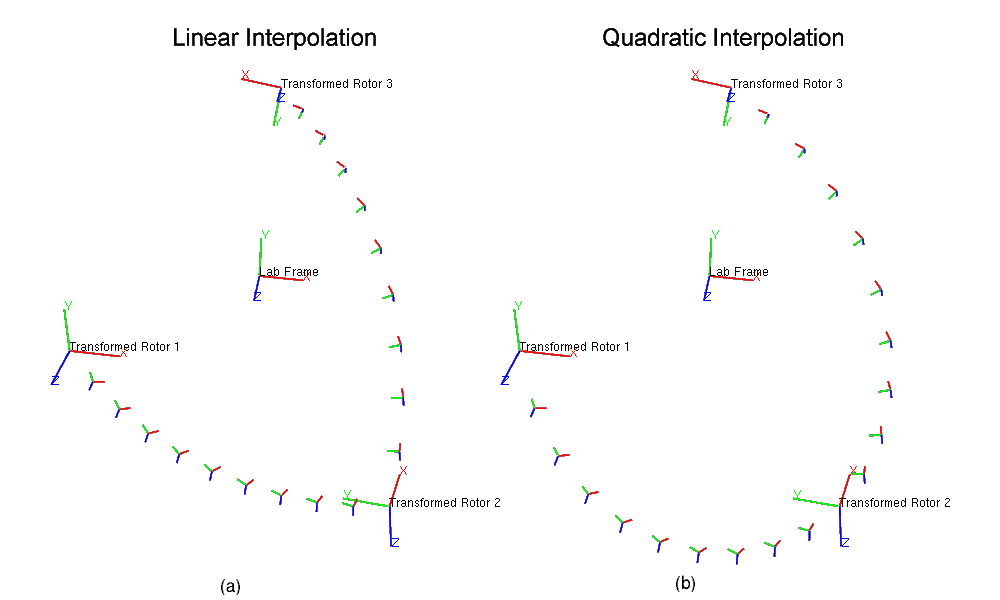
\includegraphics[width=\columnwidth]{interp}
\caption{\label{fig:interp}Examples of a) piece-wise linear and b) quadratic interpolation for
three representative poses.}
\end{figure}

\subsection{Quadratic interpolation}

Another simple form for interpolation is the quadratic interpolation where a quadratic 
is fitted through three interpolation points, $\{B_1, B_2, B_3\}$ with an interpolation
parameter varying in the range $(-1,+1)$:
\[
B'_\lambda = \left(\frac{B_3 + B_1}{2} - B_2\right)\lambda^2 + \frac{B_3 - B_1}{2}\lambda + B_2
\]
giving
\[
B'_{-1} = B_1,\quad B'_{0}=B_2\ \mbox{ and }\ B'_{+1} = B_3
\]
This interpolation varies smoothly through $B_2$ and is reflected in the final
interpolation, as shown in figure \ref{fig:interp}. Extensions to the quadratic
interpolation for more than three interpolation points, such as smoothed
quadratic interpolation \cite{cendes} are readily available.

\subsection{Alternate methods}

It is worth noting that each of the methods described above may be performed
using either direct interpolation of the bivector $\ell(R)$ corresponding
to a rotor $R$ or by interpolating the relative rotors which take one frame
to another. It is not yet clear which will give the best results and indeed
it is probably application dependent.

%%%%%%%%%%%%%%%%%%%%%%%%%%%%%%%%%%%%%%%%%%%%%%%

\section{Form of the Interpolation}

In this subsection we derive a clearer picture of the precise form of
a simple linear interpolation between two frames in order to relate the 
interpolation to existing methods used in mechanics and robotics. We will consider
the method used above whereby the rotor being interpolated takes one pose to another.

\subsection{Path of the linear interpolation}

Since we have shown that $\exp(B)$ is indeed a rotor, it follows that any
Euclidean pure-translation rotor will commute with it. Thus we only need consider the
interpolant path when interpolating from the origin to some other point since
any other interpolation can be obtained by simply translating the origin to
the start point. This location independence of the interpolation is a 
desirable property in itself but also provides a powerful analysis mechanism.

\begin{figure}\centering
\includegraphics[height=1in]{plane_basis}
\caption{\label{fig:plane_basis}Orthonormal basis resolved relative to $P$.}
\end{figure}

We have identified in subsection \ref{subsec:form} the action of the $\exp(B)$
rotor in terms of $\psi, P, t_\parallel$ and $t_\perp$. We now investigate the resulting interpolant
path when interpolating from the origin. We shall consider the interpolant
$R_\lambda = \exp(\lambda B)$ where $\lambda$ is the interpolation co-ordinate and
varies from 0 to 1. For any values of $\psi, P, t_\parallel$ and $t_\perp$,
\[
\lambda B = \frac{\lambda \psi}{2} P + \frac{\lambda (t_\perp + t_\parallel) n}{2}
\]
from which we see that the action of $\exp(\lambda B)$ is a translation along $\lambda t_\perp$, a rotation by
$\lambda \psi$ in the plane of $P$ and finally a translation along
\[
t'_\parallel =- \sinc\left(\frac{\lambda\psi}{2}\right)
\lambda t_\parallel
\left(
\cos\left(\frac{\lambda \psi}{2}\right) -
\sin\left(\frac{\lambda \psi}{2}\right) P 
\right).
\]

We firstly resolve a three dimensional, orthonormal, basis relative to $P$ as shown in figure 
\ref{fig:plane_basis}. Here $a$ and $b$ are orthonormal vectors in the plane of $P$ and hence
$P = ab$. We may now express $t_\parallel$ as $t_\parallel = t^a a + t^b b$ where $t^{\{a,b\}}$ are suitably
valued scalars.

The initial action of $\exp(B)$ upon a frame centred at the origin is therefore to 
translate it to $\lambda t_\perp$ followed by a rotation in the plane of $P$. Due to our choice of starting
point, this has no effect on the frame's location (but will have an effect on the pose, 
see the next subsection).

%\begin{figure}\centering
%\includegraphics[width=0.3\columnwidth]{tan}
%\caption{\label{fig:tan} Geometric construction showing that $\beta_1 = \frac{\pi}{2} - \beta_2$.}
%\end{figure}

\begin{figure}\centering
\includegraphics[width=\columnwidth]{helix}
\caption{\label{fig:helix} Example of an interpolant path with the final location being given by
$t_\parallel = 4a + 6b$, $\psi = 9\pi$ and $t_\perp$ having a magnitude of 1.}
\end{figure}

Finally there is a translation along $t'_\parallel$ which, 
using $c = \cos\left(\frac{\lambda \psi}{2}\right)$ and $s = \sin\left(\frac{\lambda \psi}{2}\right)$,
can be expressed in terms of $a$ and $b$ as
\begin{eqnarray*}
t'_\parallel & = & - \frac{2s}{\lambda\psi} \lambda (t^a a + t^b b) (c - sab) \\
& = & -\frac{2s}{\psi} c (t^a a + t^b b) + s ( t^b a - t^a b) \\
& \equiv & -\frac{2s}{\psi} a (t^a c + t^b s) + b ( t^b c - t^a s).
\end{eqnarray*}
The position, $r_\lambda$, of the frame at $\lambda$ along the interpolation is therefore
\[
r_\lambda = -\frac{2s}{\psi} (a (t^a c + t^b s) + b ( t^b c - t^a s)) + \lambda t_\perp
\]
which can easily be transformed via the harmonic addition theorem to
\[
r_\lambda = -\frac{2s}{\psi} \alpha \left[ a \cos\left(\frac{\lambda\psi}{2} + \beta_1\right) + b \cos\left(\frac{\lambda\psi}{2} + \beta_2\right) \right] + \lambda t_\perp
\]
where $\alpha^2 = (t^a)^2 + (t^b)^2$, $\tan \beta_1 = - \frac{t^b}{t^a}$ and $\tan \beta_2 = - \frac{-t^a}{t^b}$. 
%Figure \ref{fig:tan} is a geometric construction which clearly shows by similar figures and triangle
%identities 
It is easy, via geometric construction or otherwise, to verify that this implies
that $\beta_2 = \beta_1 + \frac{\pi}{2}$. Hence $\cos(\theta + \beta_2) = - \sin(\theta + \beta_1)$. We can now express the frame's position as
\[
r_\lambda = -\frac{2\alpha}{\psi} \left[ a \sin\left(\frac{\lambda\psi}{2}\right)\cos\left(\frac{\lambda\psi}{2} + \beta_1\right) - b \sin\left(\frac{\lambda\psi}{2}\right)\sin\left(\frac{\lambda\psi}{2} + \beta_1\right) \right] + \lambda t_\perp
\]
which can be re-arranged to give
\begin{eqnarray*}
r_\lambda & = & -\frac{\alpha}{\psi} \left[ a \left(\sin\left(\lambda\psi + \beta_1\right) - \sin\beta_1\right)
+ b \left(\cos\left(\lambda\psi + \beta_1\right) - \cos\beta_1\right) \right] + \lambda t_\perp \\
& = & -\frac{\alpha}{\psi} \left[ a \sin\left(\lambda\psi + \beta_1\right)
+ b \cos\left(\lambda\psi + \beta_1\right) \right] + \frac{\alpha}{\psi} \left[
a \sin \beta_1 + b \cos \beta_1
\right] + \lambda t_\perp 
\end{eqnarray*}
noting that in the case $\psi \rightarrow 0$, the expression becomes $r_\lambda = \lambda t_\perp$ as one would
expect. Since $a$ and $b$ are defined to be orthonormal, the path is clearly some cylindrical helix with the axis of rotation passing through 
$\alpha/\psi  \left[ a \sin \beta_1 + b \cos \beta_1 \right]$.
%where the cone has an elliptical cross-subsection with major and minor axes aligned
%to $a$ and $b$ with magnitudes $\alpha |a|$ and $\alpha |b|$ respectively. 
An illustrative example, with $a$ and $b$ having
unit magnitude, is shown in figure \ref{fig:helix}. It also clearly shows the relation between the direction of
vector $t_\parallel$ and the final translation within the plane of $P$, $t'_\parallel$.

It is worth noting a related result in screw theory, Chasles' theorem, which
states that a general displacement may be represented using a screw motion
(cylindrical helix) such as we have derived. Screw theory is widely used in
mechanics and robotics and the fact that the na\"ive linear interpolation
generated by this method is indeed a screw motion suggests that
applications of this interpolation method may be wide-ranging, especially since
this method allows many other forms of interpolation, such as B\'ezier curves
or three-point quadratic to be performed with equal ease. Also the pure
rotation interpolation given by this method reduces exactly to the quaternionic
or Lie group interpolation result allowing this method to easily extend
existing ones based upon these interpolations.

\subsection{Pose of the linear interpolation}

The pose of the transformed frame is unaffected by pure translation and hence the initial
translation by $\lambda t_\perp$ has no effect. The rotation by $\lambda \psi$ in the plane,
however, now becomes important. The subsequent translation along $t'_\parallel$ also has
no effect on the pose. We find, therefore, that the pose change $\lambda$ along the 
interpolant is just the rotation rotor $R_{\lambda \psi, P}$.
